\documentclass[10.8pt,oneside,reqno]{article}
\usepackage [utf8]{inputenc}
\usepackage [a4 paper , hmargin =1.2 in ,bottom =1.5 in]{geometry}
\usepackage [parfill]{parskip}
\usepackage{hyperref}
\usepackage{fancyhdr}
\usepackage{enumitem}
\usepackage{amsmath}
\usepackage{amsthm}
\usepackage{amssymb}
\usepackage [linesnumbered,ruled,vlined]{algorithm2e}
\usepackage{listings}
\usepackage{xcolor}
\usepackage{floatrow}
\usepackage{graphicx}
\usepackage{lmodern}
\usepackage{caption}
\lstset{
   breaklines=true,
   basicstyle=\ttfamily}
\newtheorem{definition}{Definition}
\begin{document} 


\title{Outlab 2: {\LaTeX} and gdb }
\author{P. Balasubramaniam and Shubh Kumar}
\date{Autumn 2021}
\maketitle
\fancyfoot[C]{Footer}
\renewcommand{\footrulewidth}{0.8pt}
\tableofcontents
\pagestyle{fancy}
\fancyhf{}
\rhead{Software Systems Laboratory}
\lhead{200050103 - 200050134}
\cfoot{Page \thepage}

\pagebreak


\section{Basic Theory of Linear Recurrences}

We all know about the Fibonacci Sequence, given by the recurrence 

\begin{center}
    $f_{n+2} = f_{n+1}+f_{n}$ \\ 
\end{center}

and initialised as $f_0 = 0$, $f_1 = 1$. This is an instance of what is called a Linear Recurrence
Sequence, or LRS. 

\begin{definition} 
    \label{def:1}
    LRS $( u_n )_{n=0} ^{\infty}$ of order k over field $\mathbb{F}$  is the sequence determined by the recurrence 
    \begin{center}
         \begin{equation}
            \label{eq:1}
             u_{n+k} =  \sum_{j=0}^{k-1} a_j u_{n+j}
         \end{equation}  
    \end{center}
    for integers $n \geq 0$ with $ a_0, \dots, a_{k-1} \in \mathbb{F}$, $a_0 \neq 0$, and an initialization vector
    \begin{center}
        $\begin{bmatrix}
            u_0 & \dots & u_{k-1}
        \end{bmatrix}^{\intercal} \in \mathbb{F}^{k \times 1}$
    \end{center}
    
    
\end{definition}

Thanks to Definition \hyperref[def:1]{1}, when we say that we are given $( u_n )^{\infty} _{n=0}$ of order $k$ over $\mathbb{F}$, we actually mean that we are given the $2k$ constants $ a_0 , \dots a_{k-1} , u_0 , \dots , u_{k-1} \in \mathbb{F}$. \\ 

The Fibonacci sequence shows up a lot in pop culture and DSA assignments, however, the study
of LRS is a vast subject in its own right, with applications in software verification, quantum
computing, formal languages, statistical physics, combinatorics, and theoretical biology, to name
a few.

\subsection{Computing terms of an LRS}

For a fixed $k$, assuming we can do arithmetic operations in $\mathbb{F}$ in constant time, how long does it
take to compute the $n^{th}$ term of a given LRS?  

\begin{algorithm}
    \caption{Naive first attempt $\mathsf{naive}$}
    \SetAlgoLined
    \DontPrintSemicolon
    \KwData {LRS $( u_n )_{n=0} ^{\infty}$, $n$ }
    \KwResult {$u_n$}
    \If{$n < k$}{
        \Return $u_n$ \;
    }
    \Return $\sum_{j=0}^{k-1} a_j \cdot \mathsf{naive}(( u_n )_{n=0} ^{\infty},n-k+j)$ \;

\end{algorithm}

This algorithm, unfortunately, is painfully inefficient: as you can see, the number of recursive calls will be exponentially many in $n$. This immediately prompts a more “bottom-up” \footnote{Not to be confused with the drinking phrase} approach: we start from the first $k$ terms, use them to compute the next term, and iterate this way upto $n$. This takes $\mathcal{O}(n)$ iterations. 

But we can do better, in fact, we only need $\mathcal{O}( \log n)$ iterations \footnote{In complexity analysis, the base of the logarithm is implicitly taken as $2$}. 

Technically, even Algorithm \hyperref[algo:2]{2} is \textit{inefficient}: when we analyse complexity, we do it with respect to
the size of the \textit{bit representation} of the input, i.e. how many bits it takes to specify the input. An
integer $n$ takes $ \log n$ bits to represent, so the parameter for describing complexity is not $n$, but
$\eta = \log n$. 

\begin{algorithm}
    \label{algo:2}
    \caption{Bottom up dynamic programming approach $\mathsf{bottomup}$}
    
    \SetAlgoLined
    \DontPrintSemicolon
    \KwData {LRS $( u_n )_{n=0} ^{\infty}$, $n$ }
    \KwResult {$u_n$}
    \If{$n < k$}{
        \Return $u_n$\;
    }
    $\mathsf{circularArray} \gets \{u_0 ,\dots u_{k-1}\}$\;
    $\mathsf{arrayStartIndex} \gets 0$\;
    $ n_{last} \gets k-1 $\;
    \While{$n_{last} < n$ }{
        $\mathsf{nextTerm} \gets \sum_{j=0}^{k-1} a_j \cdot \mathsf{circularArray}[(\mathsf{arrayStartIndex}+j) \% k]$\;
        $\mathsf{circularArray}[\mathsf{arrayStartIndex}] \gets \mathsf{nextTerm}$\;
        $\mathsf{arrayStartIndex} \gets (\mathsf{arrayStartIndex}+1) \% k$\;
        $n_{last} \gets n_{last} + 1$\;
    }
    \Return $\mathsf{circularArray}[(\mathsf{arrayStartIndex}+k-1) \% k]$\;

\end{algorithm}


Yes, we can compute the $n^{\text{th}}$ term with $\mathcal{O}(\eta)$ operations, and the trick here is a method called \textbf{iterated squaring.}
Given an LRS $( u_n )^{\infty} _{n=0}$, define its companion matrix $\mathbf{M} \in \mathbb{F}^{k \times k}$  as 
\begin{center}
\begin{equation}    
    \label{eq:2}
    \mathbf{M} = \begin{bmatrix}
    0 & 1 & 0 & \dots & 0 \\
    0 & 0 & 1 & \dots & 0 \\
    \vdots & \vdots & \vdots & \ddots & \vdots \\
    0 & 0 & 0 & \dots & 1 \\
    a_0 & a_1 & a_2 & \dots & a_{k-1}
    \end{bmatrix}
\end{equation} 
\end{center}
Compare equations \hyperref[eq:1]{1} and \hyperref[eq:2]{2} and observe that 
\begin{center}
    \begin{equation}
        \label{eq:3}
        \mathbf{M}^{n} \begin{bmatrix}
        u_0 \\
        \vdots \\
        u_{k-1}
    \end{bmatrix} = \begin{bmatrix}
        u_n \\
        \vdots \\
        u_{n+k-1}
    \end{bmatrix}\end{equation}
\end{center}  

Iterated squaring hinges on this ridiculously trivial observation: consider the (unique!) binary representation of $n$: if you append a $0$ to it, it becomes $2n$, if you append a $1$, it becomes $2n + 1$. 

Given $\mathbf{M}$, to compute $\mathbf{M}^{n}$, all we have to do is start with $\mathbf{I}$, read the binary representation of $n$ from most to least significant: if at some point we have $\mathbf{M}^j ,\mathbf{M}^j \cdot \mathbf{M}^j = \mathbf{M}^{2j}, \mathbf{M}^{2j} \cdot \mathbf{M} = \mathbf{M}^{2j+1}$ 

In Algorithm \hyperref[algo:3]{3}, we use a data structure called a \textbf{stack}. The constant time operations it supports are 

\begin{itemize}
    \item pushing an element onto the top of the stack
    \item popping an element from the top of the stack (i.e. deleting the topmost element)
    \item reading the topmost element
    \item checking whether the stack is empty
\end{itemize}

As you can see, it’s Last In, First Out. 

The division while loop gets the bits of $n$ from least to most significant, the iterated square while loop uses the bits from most to least significant. A stack fits the bill. 

\begin{algorithm}
    \label{algo:3}
    \caption{Iterated squaring approach $\mathsf{efficient}$}
    \SetAlgoLined
    \DontPrintSemicolon
    \KwData {LRS $( u_n )_{n=0} ^{\infty}$, $n$ }
    \KwResult {$u_n$}
    $\mathsf{quotient} \gets n$\;
    $\mathsf{operationStack} \gets \{ \}$\;
    $\mathbf{M} \gets \mathsf{companion}(( u_n )_{n=0} ^{\infty})$\;
    $ \mathbf{x} \gets \begin{bmatrix} u_0 & \dots & u_{k-1} \end{bmatrix}^{\intercal}$\;
    $ \mathbf{A} \gets \mathbf{I}_{k \times k}$\;
    \While{$\mathsf{quotient} \neq 0$}{
        $\mathsf{push}(\mathsf{operationStack},\mathsf{quotient} \% 2)$\;
        $\mathsf{quotient} \gets \mathsf{quotient}/2$\;
    }
    \While{$\mathsf{operationStack} \neq \{ \}$}{
        $\mathbf{A} \gets \mathbf{A} \cdot \mathbf{A}$\;
        \If{$\mathsf{top(operationStack)}  = 1$}{
            $\mathbf{A} \gets \mathbf{A} \cdot \mathbf{M}$\;
        }
        $\mathsf{pop(operationStack)}$\;
    }
    $\mathbf{y} \gets \mathbf{Ax}$\;
    \Return $\mathbf{y}[0]$\;

\end{algorithm}

\subsection{Problems associated with LRS}
Surprisingly, the following rather simple \textit{decision problem} \footnote{Given an arbitrary input, answer a particular question about it with Yes or No}, referred to as the Skolem problem, has been open for the last eight decades or so.

\begin{definition} 
    
    (Skolem problem). For the arbitrary LRS $( u_n )^{\infty} _{n=0}$ whose description is given as input, does there exist an integer $n \geq 0$ such that $u_{n} = 0$? 

\end{definition}

This has a bunch of equivalent formulations, and by being open, we mean that nobody really knows of an algorithm that can decide it (the algorithm should terminate and give the correct answer for \textit{all} possible inputs), or whether there is such an algorithm at all.

We can also consider another related problem for LRS over fields where the $>$ operator is defined:
\begin{definition} 
    (Positivity problem). For the arbitrary LRS $( u_n )^{\infty} _{n=0}$ whose description is given as input, is it the case that for all integers $n \geq 0$, $u_{n} \geq 0$?
 \end{definition}

Deciding even special cases of these problems (i.e. restricting what kind of LRS can be fed as input) requires sophisticated maths, like Kronecker’s theorem on Diophantine approximations, \cite{topology}, [Chap. 7, Sec. 1.3, Prop. 7], and profound properties of “algebraic” numbers \cite{algebra} and then some more mathematical arsenal \cite{positivity,compgeo}.

If you found this short write up interesting, \href{https://fmindia.cmi.ac.in/update2013/presentations/S-Akshay.pdf}{here}. is a survey talk about the problem, given not so long ago.

\pagebreak

\section{Programming}
\begin{figure}[!h]
    \begin{floatrow}
      \ffigbox{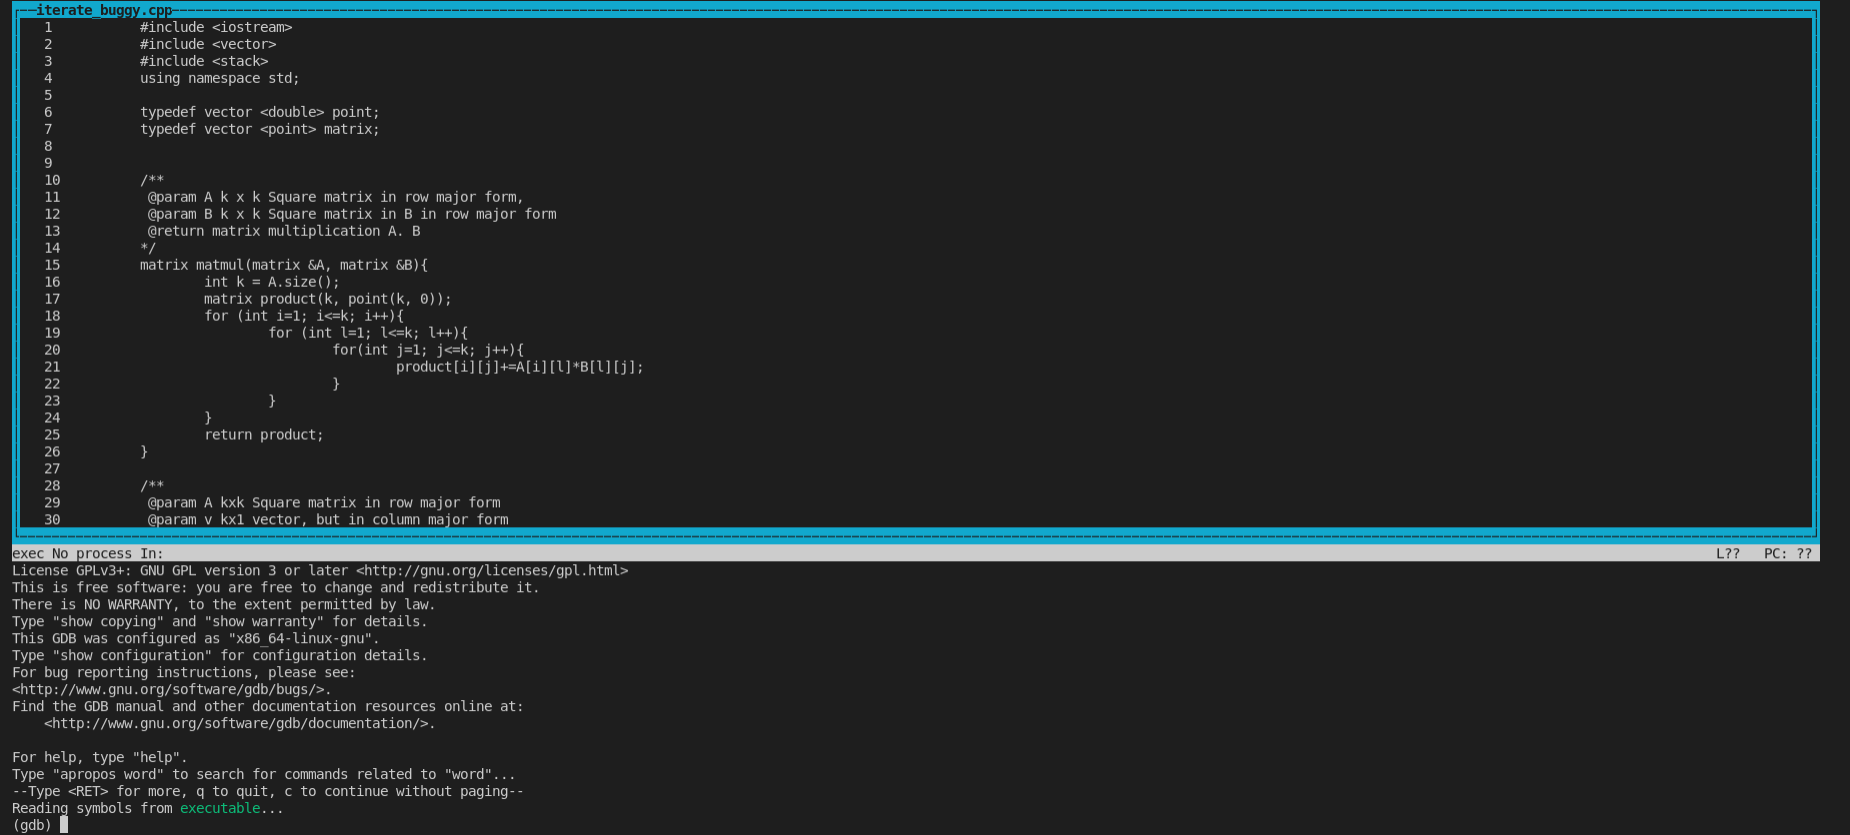
\includegraphics[scale = 0.115]{s1.png}}{\caption{Screenshot 1:gdb interface}} %replace s1.png with name of first screenshot
      \ffigbox{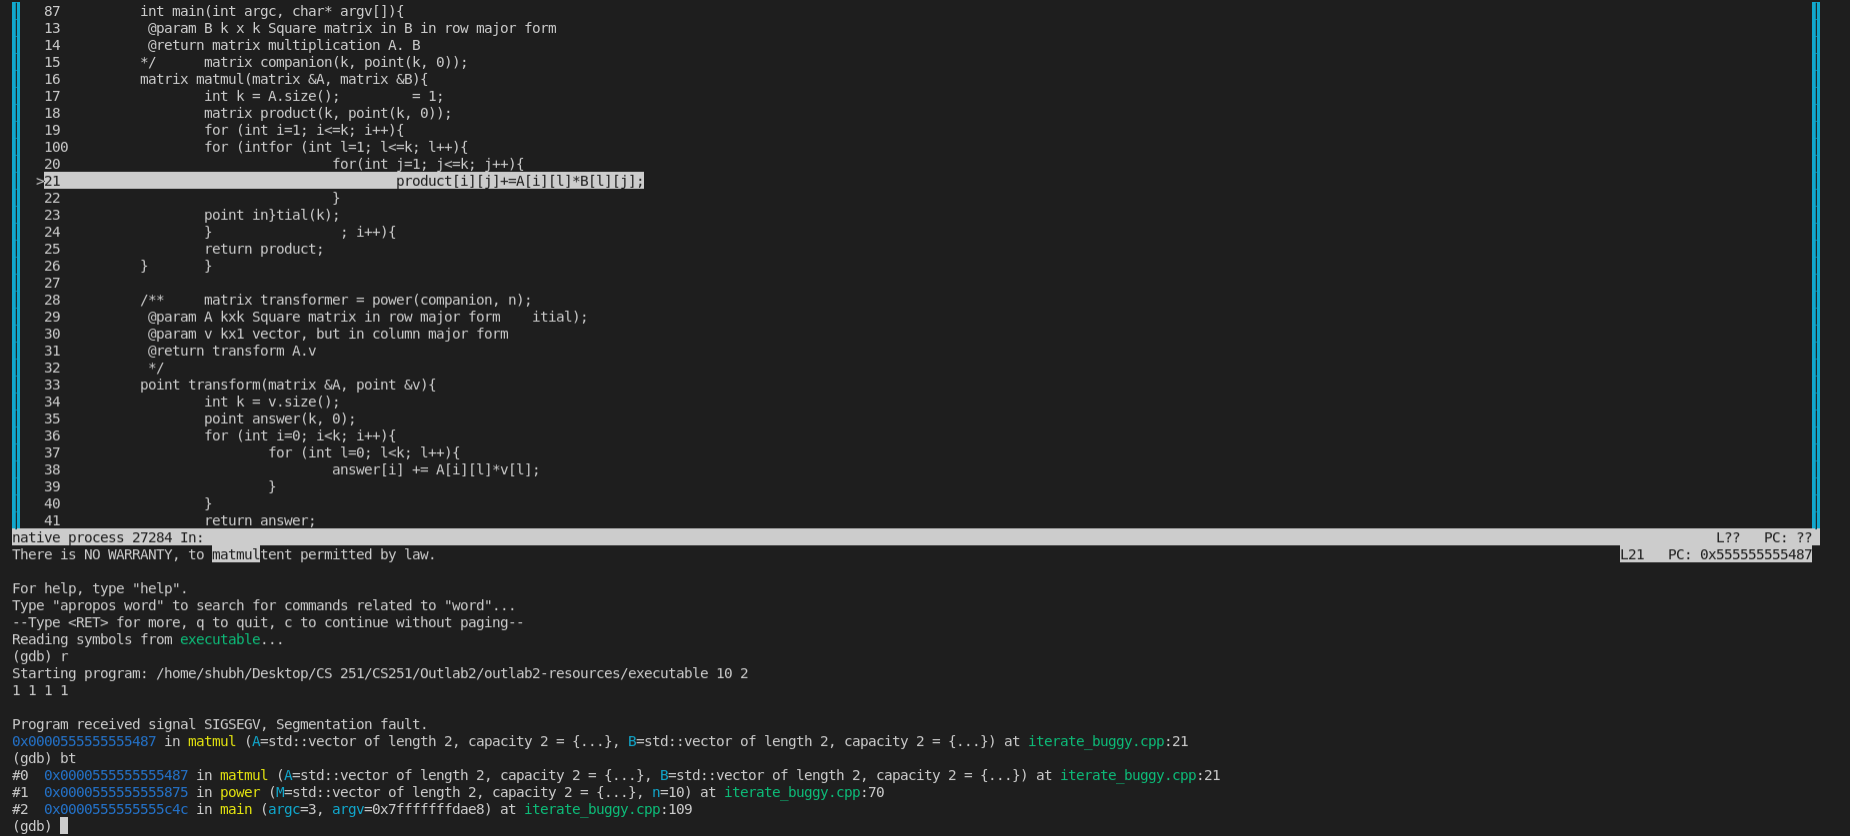
\includegraphics[scale = 0.115]{s2.png}}{\caption{Screenshot 2:gdb backtrace}} %replace s2.png with name of second screenshot
    \end{floatrow}
\end{figure}






Here, are the snippets we had to complete :  \\ 


\begin{verbatim}
    (gdb) print working
\end{verbatim}
\begin{lstlisting}

   $1 = std::vector of length 2, capacity 2 = {std::vector of length 2, capacity 2 = {1, 0}, std::vector of length 2, capacity 2 = {0, 1}}
    

\end{lstlisting}
\begin{verbatim}
    (gdb) print operations
\end{verbatim}
\begin{lstlisting}
    $2 = std::stack wrapping: std::deque with 9 elements = {0, 1, 0, 1, 1, 0, 1, 1, 1}
 \end{lstlisting}




\begin{table}[h!]
    \begin{center}
      
      \label{table1}
      \begin{tabular}{l|c} 
        \textbf{operations} & \textbf{working} \\
        \hline
        $\{ 0, 1, 0, 1, 1, 0, 1, 1, 1 \}$ & $\{ 1, 0, 0, 1 \}$\\ 
        \hline
        $\{ 0, 1, 0, 1, 1, 0, 1, 1 \}$ & $\{ 0, 1, 1, 1 \}$ \\ 
        \hline
        $\{ 0, 1, 0, 1, 1, 0, 1 \}$ & $\{ 1, 2, 2, 3 \}$ \\ 
        \hline
        $\{ 0, 1, 0, 1, 1, 0 \}$ & $\{ 8, 13, 13, 21 \}$ \\ 
        \hline
        $\{ 0, 1, 0, 1, 1 \}$ & $\{ 233, 377, 377, 610 \}$ \\ 
        \hline
        $\{ 0, 1, 0, 1 \}$ & $\{317811, 514229, 514229, 832040 \}$ \\ 
        \hline %%%%
        $\{ 0, 1, 0 \}$ & $\{591286729879, 956722026041, 956722026041, 1548008755920 \}$ \\ 
        \hline
        $\{ 0, 1\}$ & $\{ 1.26e+24, 2.04e+24, 2.04e+24, 3.31e+24 \}$ \\ 
        \hline
        $\{ 0 \}$ & $\{ 9.36e+48, 1.51e+49, 1.51e+49, 2.45e+49 \}$ \\ 
        \hline
        $\{ \}$ & $\{ 3.17e+98, 5.13e+98, 5.13e+98,8.31e+98 \}$ \\ 
        \hline
        
      \end{tabular}
      \caption{operations vs. working}
    \end{center}
  \end{table}
  
  \pagebreak
  
 
\section{Hints and Tips}
\label{Listing:2}
\begin{center}
    \textbf{\Large Listing 2: [LaTeX]TeX} \\
    \textbf{Packages imported in the original} \\
\end{center}
\lstset
{
    language=[LaTeX]TeX,
    breaklines=true,
    basicstyle=\tt\scriptsize,
    keywordstyle=\color{blue},
    numbers=left,
    numberstyle=\tiny\color{gray}
}
\begin{lstlisting}
    \documentclass{article}
    \usepackage[utf8]{inputenc}
    \usepackage[a4paper,hmargin=1.2in,bottom=1.5in]{geometry}
    \usepackage[parfill]{parskip}
    \usepackage{hyperref}
    \usepackage{fancyhdr}
    \usepackage{enumitem}
    \usepackage{amsmath}
    \usepackage{amsthm}
    \usepackage{amssymb}
    \usepackage[linesnumbered,ruled,vlined]{algorithm2e}
    \usepackage{listings}
    \usepackage{xcolor}
    \usepackage{floatrow}
    \usepackage{graphicx}
    \bibliographystyle{plainurl}
    \bibliography{biblio}
\end{lstlisting}

\begin{thebibliography}{9}

\bibitem{positivity} 
J. P. Bell and S. Gerhold. On the positivity set of a linear recurrence.
\textit{Israel Jour. Math}, 
57, 2007.

\bibitem{topology} 
N. Bourbaki.
\textit{Elements of Mathematics: General Topology (Part 2)}. 
Addison-Wesley, 1966.

\bibitem{algebra} 
M. Mignotte. Some useful bounds. In 
\textit{Computer Algebra}, 
1982.

\bibitem{compgeo}

James Renegar. On the computational complexity and geometry of the first-order theory of the reals, part i: Introduction. preliminaries. the geometry of semi-algebraic sets. the decision problem for the existential theory of the reals. 
\textit{J. Symb. Comput.},
13:255–300, 1992.

\bibitem{listing2}
Reference to Listing \color{blue}\hyperref[Listing:2]{2}

\end{thebibliography}

\end{document}